\documentclass{beamer}
\usepackage[utf8]{inputenc}
\usepackage{graphicx}
\usetheme{Madrid}
\usecolortheme{wolverine}

\title {K Plus Proches Voisins}
\subtitle{Analyse de temps de calcul - Avec 2 méthodes}

\author{Roche Anaïs \and Yildiz Tolga}

\date {22 mai 2023}

\AtBeginSection[]
{
  \begin{frame}
    \frametitle{Sommaire}
    \tableofcontents[currentsection]
  \end{frame}
}

\begin{document}

\frame{\titlepage}

\begin{frame}
\frametitle{Sommaire}
\tableofcontents
\end{frame}

\section{Analyse du temps de calcul en fonction du nombre de points pour k-ppv fixe}

\begin{frame}
\frametitle{Analyse pour k-ppv fixe}
\begin{columns}
    \column{0.5\textwidth}
    \begin{figure}
      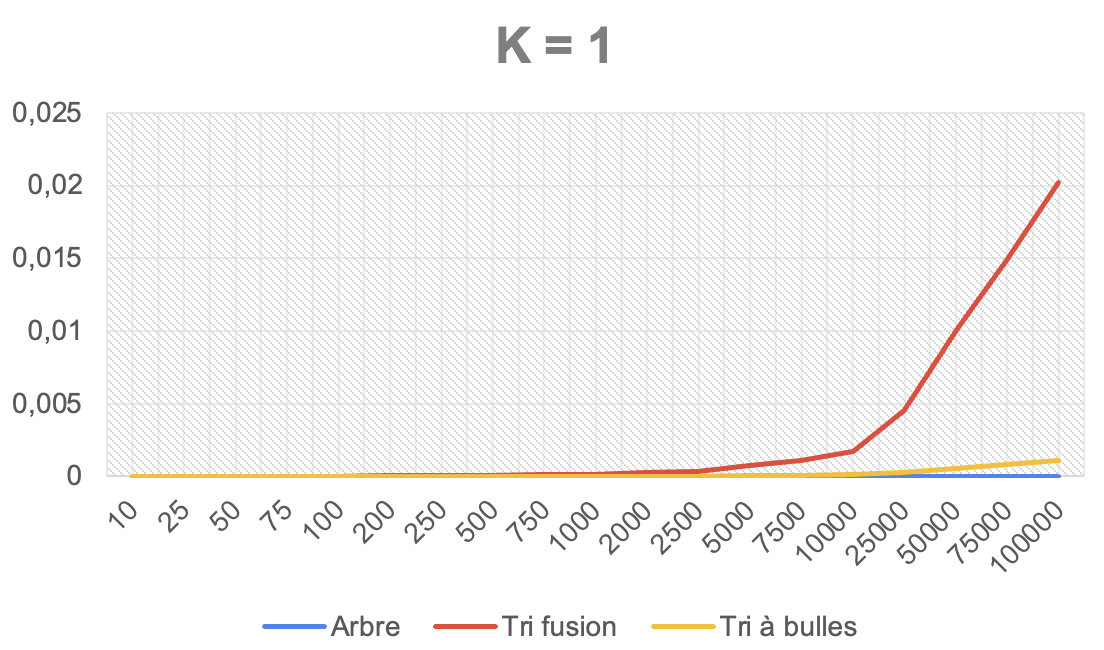
\includegraphics[width=\textwidth]{Beamer/K_1.png}
    \end{figure}

    \column{0.5\textwidth}
    \begin{figure}
      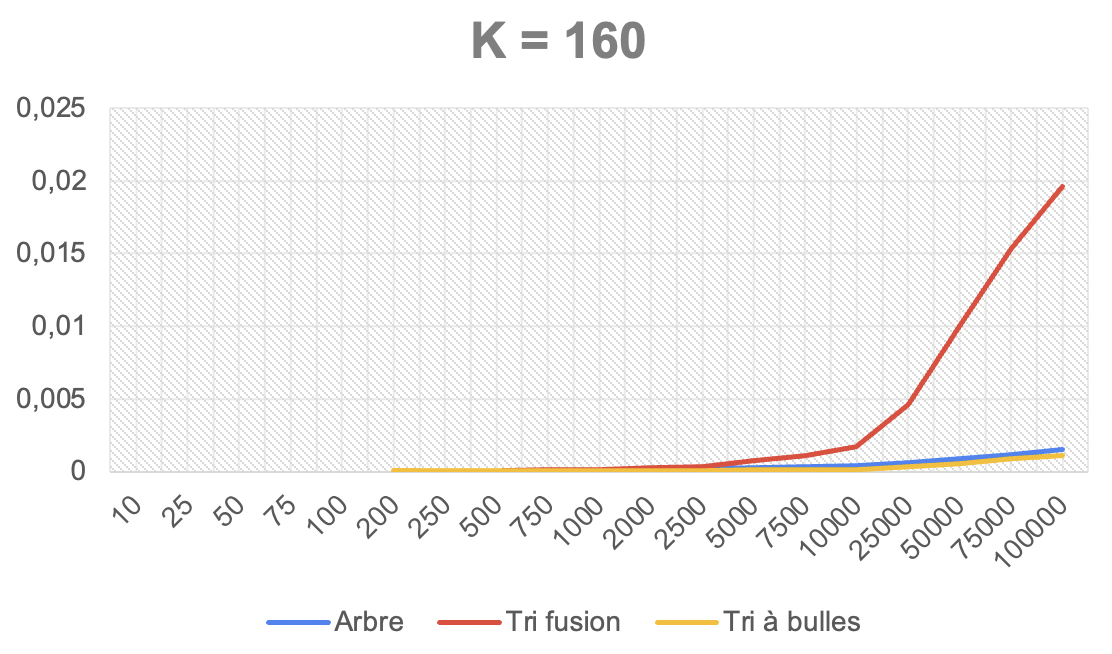
\includegraphics[width=\textwidth]{Beamer/K_160.png}
    \end{figure}
\end{columns}

  \begin{columns}
    \column{0.5\textwidth}
    \begin{figure}
      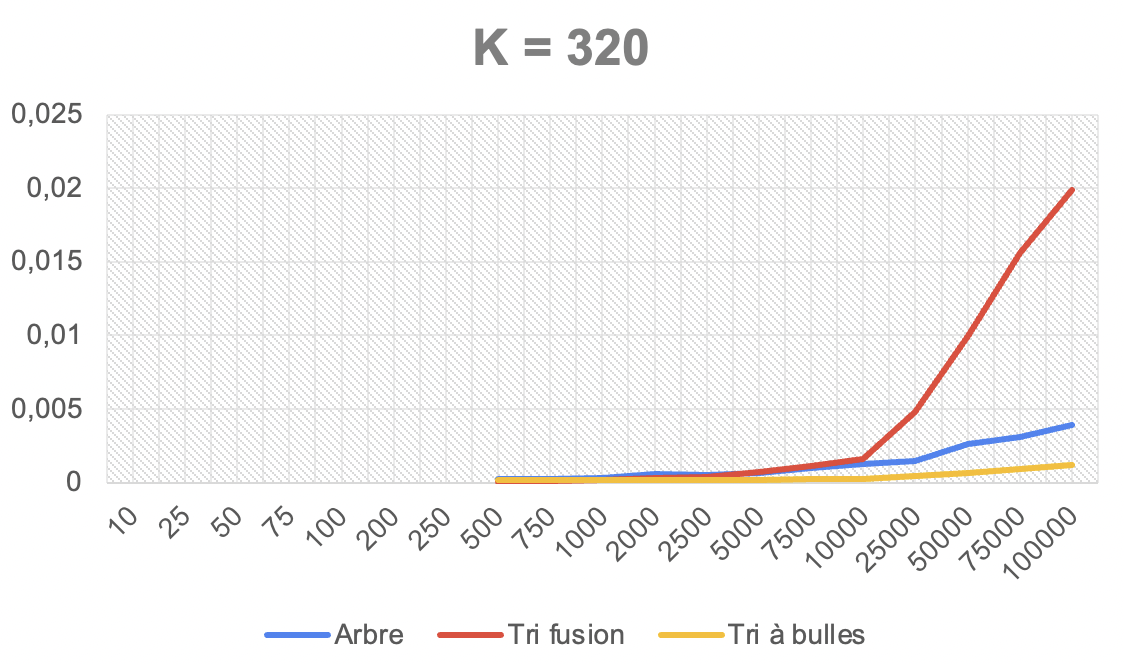
\includegraphics[width=\textwidth]{Beamer/K_320.png}
    \end{figure}

    \column{0.5\textwidth}
    \begin{figure}
      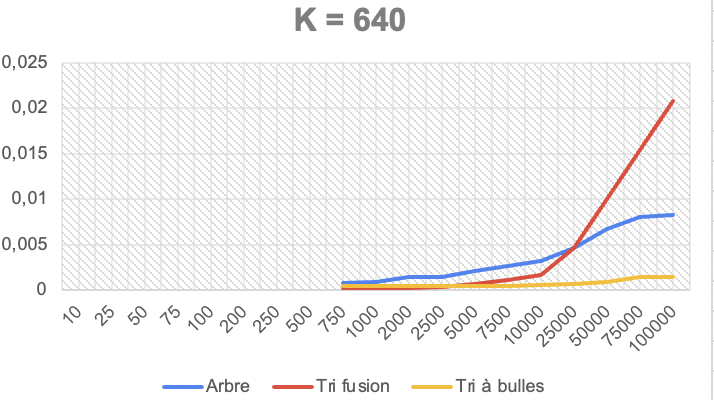
\includegraphics[width=\textwidth]{Beamer/K_640.png}
    \end{figure}
\end{columns}
\end{frame}

\begin{frame}
\begin{columns}
    \column{0.5\textwidth}
    \begin{figure}
      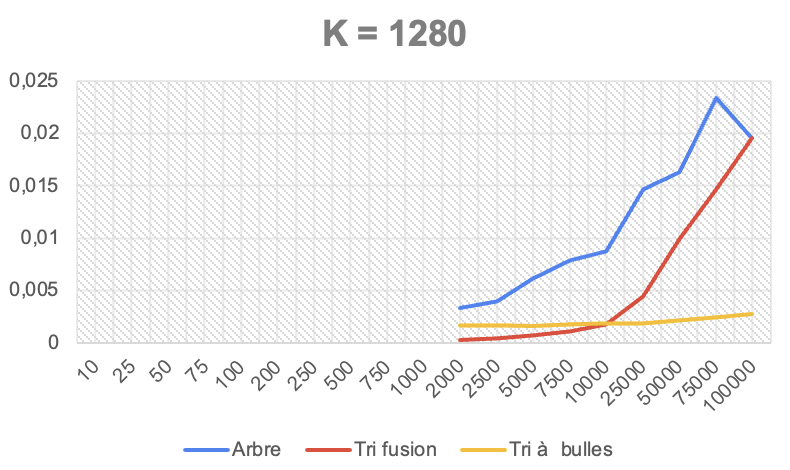
\includegraphics[width=\textwidth]{Beamer/K_1280.png}
    \end{figure}

    \column{0.5\textwidth}
    \begin{figure}
      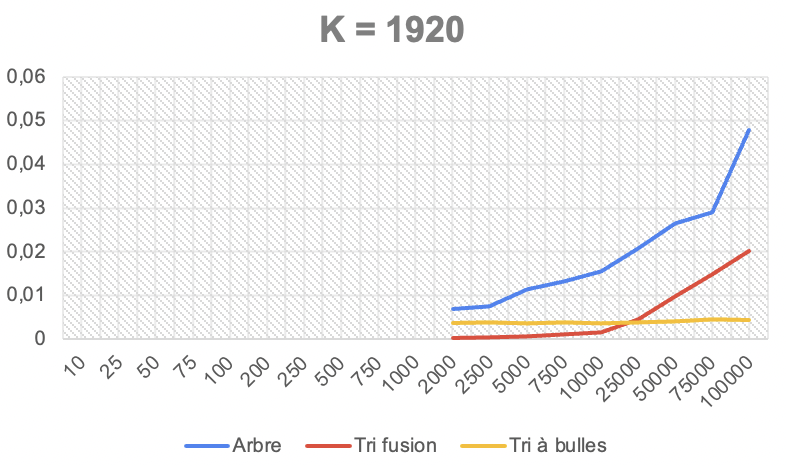
\includegraphics[width=\textwidth]{Beamer/K_1920.png}
    \end{figure}
\end{columns}

\begin{block}{Conclusion pour k-ppv fixe}
Privilégier l'arbre pour un nombre de points faible pour un k-ppv fixe et le tri à bulles ainsi que le tri fusion pour un nombre de points élevé.
\end{block}
\end{frame}

\section{Analyse du temps de calcul en fonction de k-ppv pour un nombre de points fixe}

\begin{frame}
\frametitle{Analyse pour nombre de points fixe}
\begin{columns}
    \column{0.5\textwidth}
    \begin{figure}
      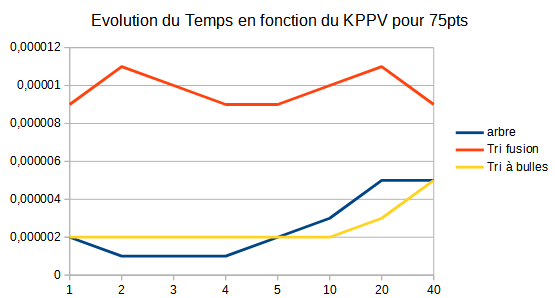
\includegraphics[width=\textwidth]{Beamer/K_75_M2.png}
    \end{figure}

    \column{0.5\textwidth}
    \begin{figure}
      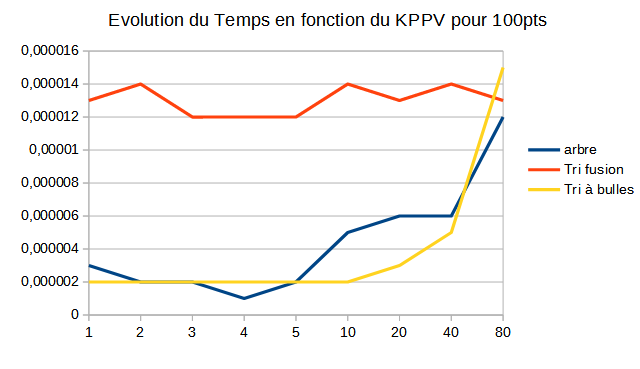
\includegraphics[width=\textwidth]{Beamer/K_100_M2.png}
    \end{figure}
\end{columns}

  \begin{columns}
    \column{0.5\textwidth}
    \begin{figure}
      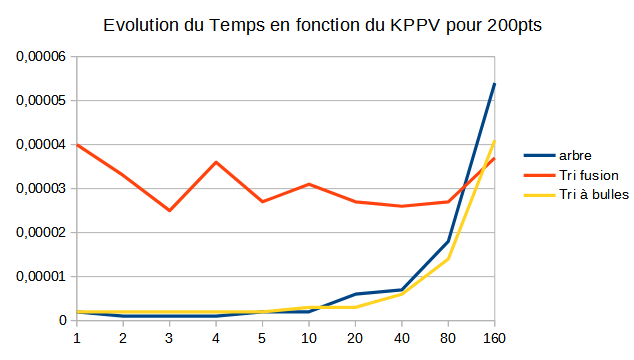
\includegraphics[width=\textwidth]{Beamer/K_200_M2.png}
    \end{figure}

    \column{0.5\textwidth}
    \begin{figure}
      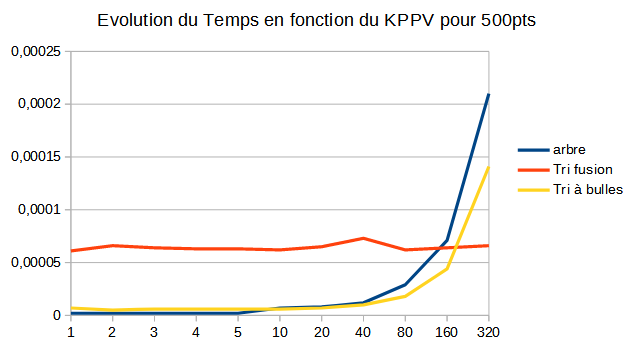
\includegraphics[width=\textwidth]{Beamer/K_500_M2.png}
    \end{figure}
\end{columns}
\end{frame}

\begin{frame}
\begin{figure}
      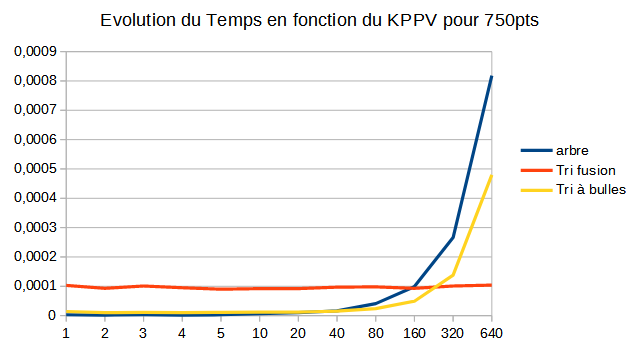
\includegraphics[width=\textwidth]{Beamer/K_750_M2.png}
\end{figure}
\begin{block}{Conclusion pour nombre de points fixe}
Pour un k-ppv important privilégier le tri fusion.
\end{block}
\end{frame}

\section{Analyse de l'ecart type pour k-ppv fixe}

\begin{frame}
\frametitle{Analyse ecart type pour k-ppv fixe}
\begin{columns}
    \column{0.5\textwidth}
    \begin{figure}
      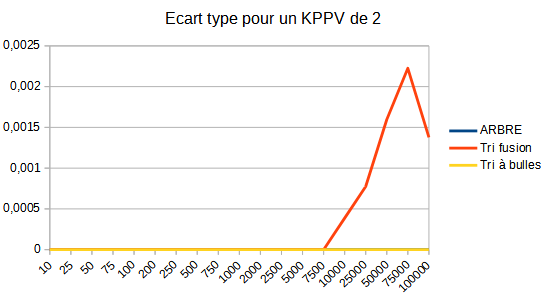
\includegraphics[width=\textwidth]{Beamer/ET_KPPV_2.png}
    \end{figure}

    \column{0.5\textwidth}
    \begin{figure}
      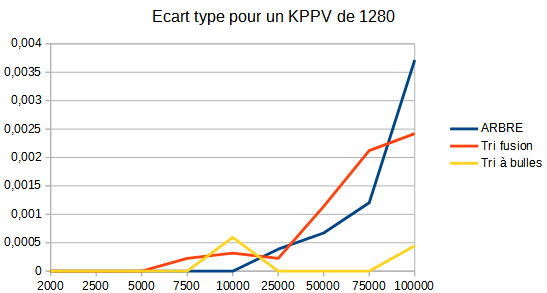
\includegraphics[width=\textwidth]{Beamer/ET_KPPV_1280.png}
    \end{figure}
\end{columns}

  \begin{columns}
    \column{0.5\textwidth}
    \begin{figure}
      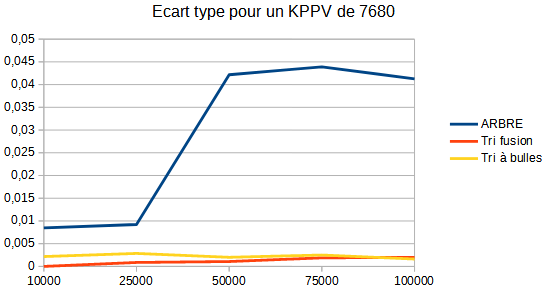
\includegraphics[width=\textwidth]{Beamer/ET_KPPV_7680.png}
    \end{figure}

    \column{0.5\textwidth}
    \begin{figure}
      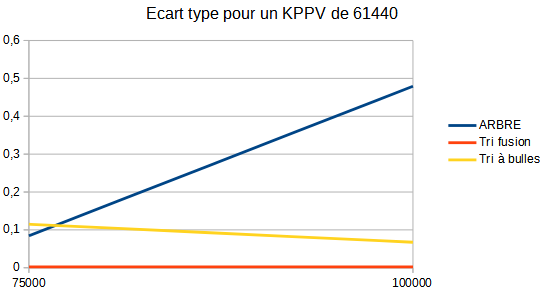
\includegraphics[width=\textwidth]{Beamer/ET_KPPV_61440.png}
    \end{figure}
\end{columns}
\end{frame}

\section{Analyse de l'ecart type pour nombre de points fixe}

\begin{frame}
\frametitle{Analyse de l'ecart type pour nombre de points fixe}
\begin{columns}
    \column{0.5\textwidth}
    \begin{figure}
      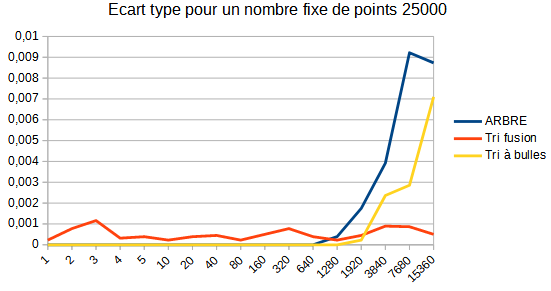
\includegraphics[width=\textwidth]{Beamer/ET_NB_25000.png}
    \end{figure}

    \column{0.5\textwidth}
    \begin{figure}
      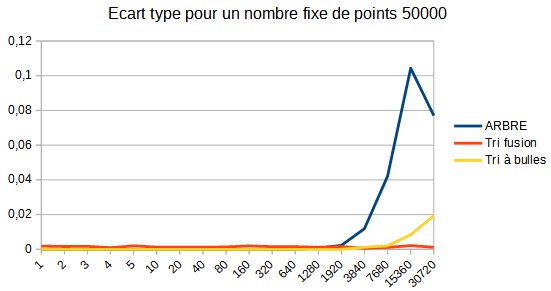
\includegraphics[width=\textwidth]{Beamer/ET_NB_50000.png}
    \end{figure}
\end{columns}

  \begin{columns}
    \column{0.5\textwidth}
    \begin{figure}
      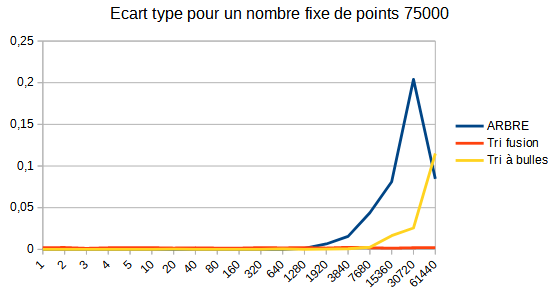
\includegraphics[width=\textwidth]{Beamer/ET_NB_75000.png}
    \end{figure}

    \column{0.5\textwidth}
    \begin{figure}
      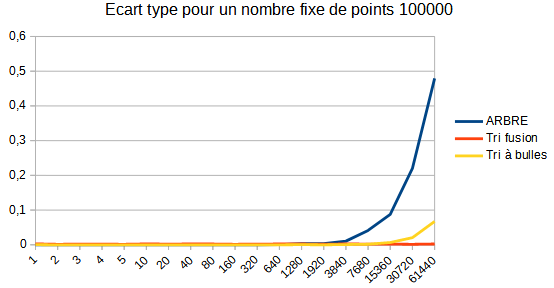
\includegraphics[width=\textwidth]{Beamer/ET_NB_100000.png}
    \end{figure}
\end{columns}
\end{frame}

\section{ Conclusion générale}

\begin{frame}
\frametitle{Conclusion}
\begin{itemize}
    \setlength\itemsep{3em}
    \item[{\color{blue}\textbullet}] Pour un petit nombre de k-ppv : l'arbre est plus performant.
    \item[{\color{blue}\textbullet}] Pour un grand nombre de k-ppv : le tri fusion est plus performant.
\end{itemize}
\end{frame}

\end{document}


